\documentclass[11pt]{article}
    %	options include 12pt or 11pt or 10pt
    %	classes include article, report, book, letter, thesis

    \usepackage{amsmath}
    \usepackage{array}
    \setlength\extrarowheight{2pt}
    \usepackage{graphicx}
    \usepackage{epstopdf}
    \usepackage{graphics}
    \graphicspath{ {/home/shanedrafahl/coms331/hw0} }
    
    \title{HW3}
    \author{Shane Drafahl}
    \date{26 September,2017}

    \begin{document}
    \maketitle

    1. (a) 

    \begin{figure}[!htb]
        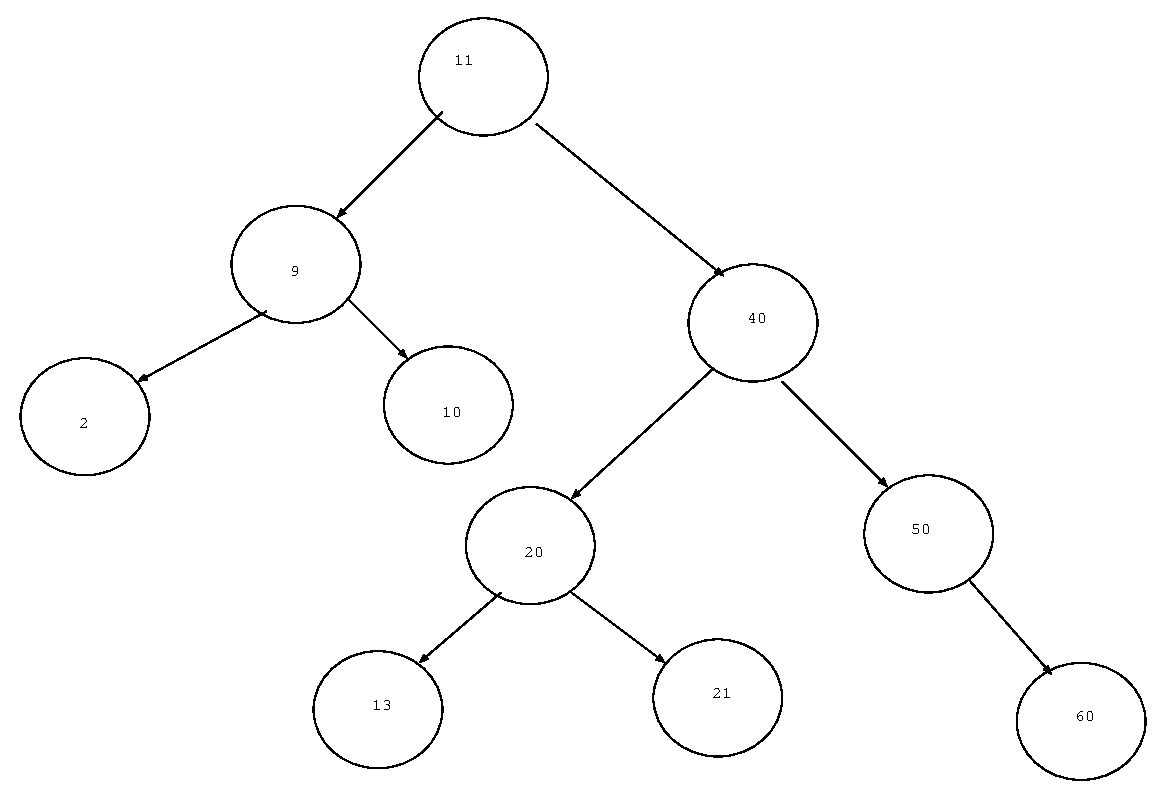
\includegraphics[scale=.7]{./unbalanced.eps}
    \end{figure}
    
    $ \newline \newline $

    (b).
        Every node in this tree follows the requirements to be an AVL tree. Every node
        has a difference of height for it children that is either -1,0,1.

        $ \newline \newline $

    (c).
        $ (2x + 3) $ mod $ 5 \leq 4 $ so we can assume the hashset only has a size of 4.
        
        $ \newline \newline $
        \begin{figure}[!htb]
            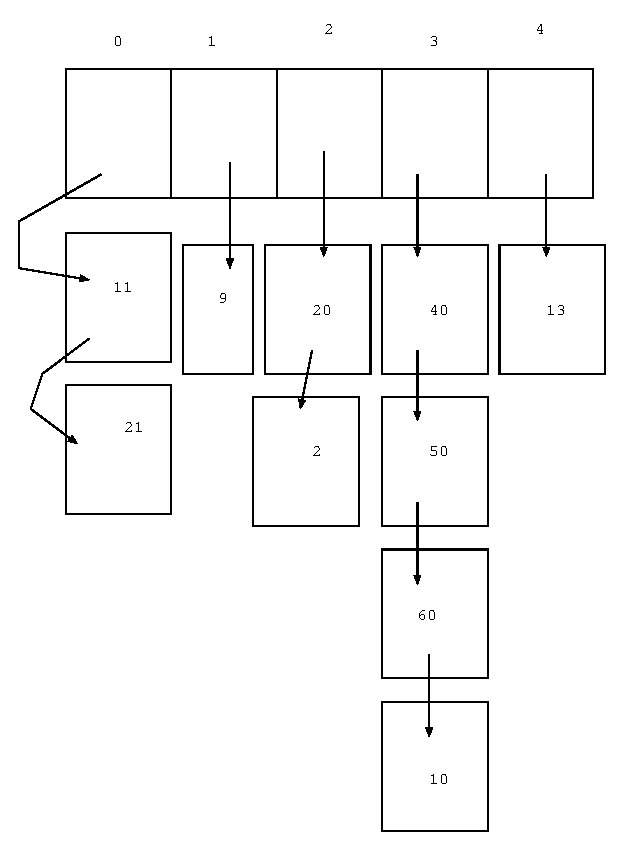
\includegraphics[scale=.7]{./hash.eps}
        \end{figure}
        
        $ \newline \newline $

        2. Consider that binary tree T is a perfectly balanced tree so each node must
        have 2 children or 0 children. The tree has $ n = 2^{ \ell } - 1 $ 
        distinct integers so the tree must have n nodes.
        
        $ \newline $

        Lemma $ n = 2^{h + 1} - 1 $ where h is the height of the binary tree.

        $ \newline $

        Basis: Suppose a tree $ T^{'} $ has only a single root node so h = 0.
        $ 1 = 2^{1} - 1 $.

        $ \newline $

        Inductive Hypothesis: 
        Suppose that $ n = 2^{h + 1} - 1 $ is true for tree $T_{1}$, $T_{2}$.

        $ \newline $

        Recursion:

        Using structural induction for $ T_{1} $, $ T_{2} $
        returns the number of node for each tree $ n = 2^{h + 1} - 1 $ where
        h is the height for either tree. Both trees need to have the same 
        height or else the new binary tree might not be perfectly balanced .
        If we combine $ T_{1} $ and $ T_{2} $ and for order it to be a perfectly balanced tree
        we will add a single node N that will be the new root node that is a parent
        with the roots from $ T_{1} $ and $ T_{2} $. The height of the new tree 1 + h 
        the number of nodes. The number of nodes in the new tree will be 
        $ 2^{h + 1} - 1 $ + $ 2^{h + 1} - 1 $ + 1 or it can be reduced to 
        $ 2^{h + 2} - 2 + 1$ ... $ n = 2^{h + 2} - 1 $. Since $ 1 + h = h^{'}$
        the new tree will have $ 2^{h^{'} + 1} - 1 $ nodes. So therefore for all 
        perfectly balanced trees there are $ 2^{h + 1} - 1 $ nodes for its height h.
        QED

        $ \newline $

        $ n = 2^{ \ell } - 1 $ is the number of nodes in the tree so therefore 
        $ \ell $ = h + 1 where h is the height of the tree. 
        
        $ \newline $

        The algorithm is 

        \begin{verbatim}
            // T is a tree
            // T.R is the root node
            // T.R.L is the left child of the root
            // T.R.R is the right child of the root

            getElementSmallerThan(T) {
                return T.R.R
            }

        \end{verbatim}

        $ \newline $

        This algorithm is obviously O(1) this algorithm is correct because 
        by the lemma there are $ 2^{h + 1} - 1 $ nodes in the tree and we want a 
        value that is smaller than $ 2^{h - 1} - 1 $ nodes. If there are $ a $ 
        nodes in the tree then we need to find the node smaller than 
        $ \frac{a + 1}{4} - 1 $ nodes. Notice that $ \frac{a + 1}{4} - 1 $
        equals the number of nodes in the subtree of the right child of the 
        right child of the root node. This makes sense because it should be
        about a fourth of the nodes it needs to be smaller than. For a tree
        of three nodes the right child has no children so $ \frac{3 + 1}{4} - 1 $ = 0
        so in that case the right child of the root would be the largest
        value in the tree being smaller than 0 values in the tree. For larger
        trees almost a quarter of the entire tree is the subtree of the right child of the
        right child of the root. Meaning that the right child of the root is smaller than
        $ 2^{ \ell - 2 } - 1 $ or $ n = 2^{ h - 1 } - 1 $ elements in the tree. QED
        
        $ \newline \newline $

        (b) We start with a tree that looks like
        \begin{figure}[!htb]
            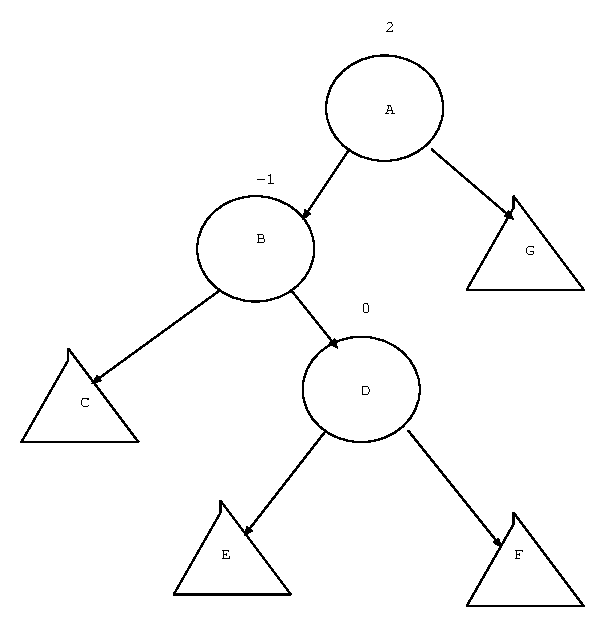
\includegraphics[scale=.7]{./preBalanced.eps}
        \end{figure}

        $ \newline \newline $
        Suppose that tree C has a height of $ h^{'} $, E and F has a height of $ h $ and G has a height of 
        $ h^{''} $. B has a balance factor of -1 so $ ( h^{'} + 1 ) - (h + 2) = -1 $ so $ h^{'} = h $.
        A has a balance factor of 2 so that means that $ (h + 3) - (h^{''} + 1) = 3 $ so $ h = h^{''} $.
        $ \newline \newline $
        So because the D is less than a and greater than B we will rotate the D.
        
        \begin{figure}[!htb]
            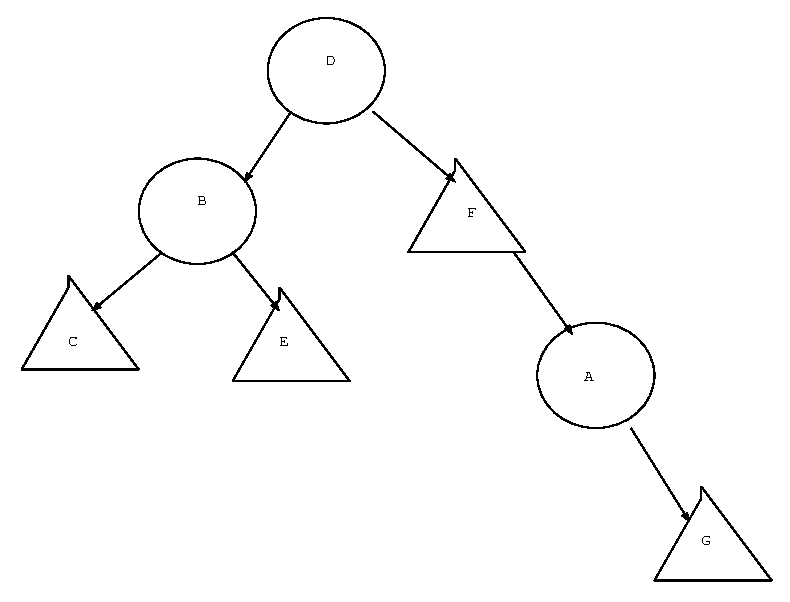
\includegraphics[scale=.7]{./preBalanced2.eps}
        \end{figure}

        $ \newline \newline $

        This tree is still not balanced. So we will rotate a subtree to get.
 
        \begin{figure}[!htb]
            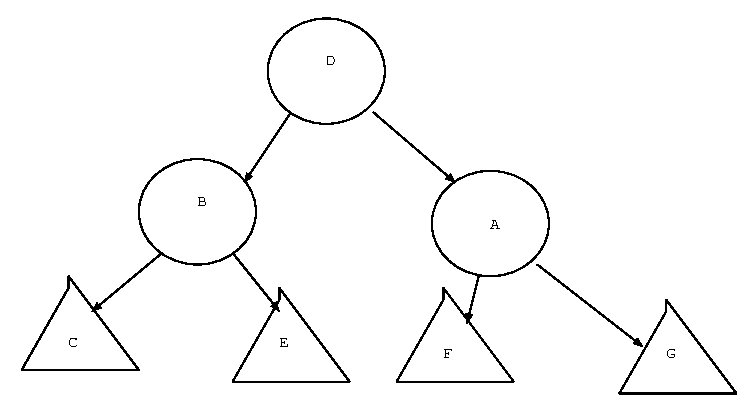
\includegraphics[scale=.7]{./preBalanced3.eps}
        \end{figure}     

        $ \newline $

        The balance factor for D,B,A are 0 each. It is a perfectly balanced tree.

        $ \newline $

        3. In order to do this I will create a tree of the right size. Since $ 2^{h} = l $ where the h is 
        the height of the tree and l is the number of leaves .I just need to create a tree of that size and then
        insert the values into the leaf nodes. $ 2^{h + 1} - 1 $ also equals the number of nodes in the tree.  

        \begin{verbatim}
        
        Node {
            value = 0,
            Node parent,
            Node leftChild,
            Node rightChild,
        }

        Tree {
            Node root,
            List leafNodes,
        }

        function createTree(List list) {
            Tree tree
            tree.root
            Node root
            root.parent = null
            tree.root = root
            height = log2(list.length)
            List leafNodes = [] // empty list that will hold nodes
            tree.leafNodes = leafNodes
            addLayerToTree(root, 0, height, leafNodes)
            addValuesToLeaves(list, leafNodes)
            return tree
        }

        function addLayerToTree(Node n, level, height,List leafs) {
            if(level != height) {
                Node left
                Node right
                n.leftChild = left
                n.rightChild = right
                addLayerToTree(n.leftChild, level + 1, height)
                addLayerToTree(n.rightChild, level + 1, height)
            } else {
                leafs.add(n)
            }
        }

        function addValuesToLeaves(List values,List nodes) {
            for(int x=0;x<values.length;x++) {
                Node node = nodes.get(x)
                value = values.get(x)
                node.value = value
            }
        }

        \end{verbatim}

        This algorithm creates a binary tree to the correct height it would need to be for there to be at least a single leaf node 
        node per value. Because of the order of recursion we know the list of nodes that is given to addValuesToLeaves() will
        be in order from left to right. To determine the runtime of the algorithm we first observe that the atomic lines
        dont matter so we will focus on the two functions. addValuesToLeaves() is $ O(n) $ if n was equal to the number 
        of items in the list. Now we will look at addLayerToTree, it is a recursive function so we must observe how many iterations
        it would be called in terms of n before it reaches the base case. The function goes untill the level != height. 
        The height $ log_{2}(n) = h $.The level increases by 1 every recursive call so this function is called  $ log_{2}(n) + 1 $ times.
        So the runtime of the whole algorithm is $ n + log_{2}(n) + 1 = O(n) $.

        $ \newline $
        
        (b) For this problem we will use a binary search tree but then store the sum in its parent nodes. So we will
        modify the data structure in the first part. We need a function to assign the sum values to the non leaf nodes.


        $ \newline $

        \begin{verbatim}
        
        // new function
        function assignSums(Node n) {
            if(n.parent !=null) {
                n.parent.value += n.value
                assignSums(n.parent)
            }
        }

        // modify this function

        function createTree(List list) {
            Tree tree
            tree.root
            Node root
            root.parent = null
            tree.root = root
            height = log2(list.length)
            List leafNodes = [] // empty list that will hold nodes
            addLayerToTree(root, 0, height, leafNodes)
            addValuesToLeaves(list, leafNodes)
            for(int x=0;x<leafNodes.length;x++) {
                assignSums(leafNodes.get(x))
            }
            return tree
        }

        // one of the required functions 
        function increment(i , val) {
            Tree t // the tree the algorithm is applied to
            recursiveIncrament(t.leafNodes.get(i), val)
        }

        function recursiveIncrament(Node node, value) {
            node.value += value
            if(node.parent != null) {
                recursiveIncrament(node.parent, value)
            }
        }

        SS() {
            Tree t // the tree the algorithm is applied to
            return t.root.value
        }

        \end{verbatim}

        The datastructure is a tree structure that the leaf nodes hold the values and the shared parents are the sum of each of its
        child nodes. Similar to a fibonacci tree. The root node therefore holds the sum for all values in the tree. 
        The time bounds for SS() = $ O(1) $ and increment(i, val) adds a value to the leaf node and then recursively
        travels up the tree untill it reaches the root of the tree. The height of the tree is the log of the number of leaf nodes
        so we know if n represents the number of leaf nodes that it would have take $ log(n) $ steps to perform recursiveIncrament so 
        therefore increment = $ O(log(n)) $.

        $ \newline \newline $

        4. This can be accomplished with a Red and Black binary search tree.


        \begin{verbatim}
        
    D {
        Node root,
        Node lastAdded,
        List leafNodes,
    }

    Node {
        color,
        value = 0,
        quantity = 0,
        Node parent,
        Node leftChild = null,
        Node rightChild = null,

    }

    function getBalance(Node n) {
        return (getHeight(n.left) - getHeight(n.right));
    }


    function insert(D structure, val)
    {
        Node n
        n.value = val
        if(structure.root != null) {
            n.color = RED
            structure.root = n
        } else {
            Node root = structure.root
            recursiveInsert(structure, root, n);
            balanceTree(structure);
            while (n.parent != null) {
                n = n.parent
            }
            structure.root = n;
        }
    }

    function remove(D structure, k) {
        
        recurseFindAndDelete(structure, k, structure.root)
    }

    function recurseFindAndDelete(D structure, k, Node n) {
        Node root = structure.root
        left = getHeight(root.left)
        right = getHeight(root.right)

    }

    function getQuantity(Node n, height) {
        if(n.right != null) {
            height++
            getHeight(n.right)
        } else {
            if(n.left != null) {
                height++
                getHeight(n.left)
            } else {
                return height
            }
        }
        
    }


    function recursiveInsert(D structure, Node root, Node n) {
        if (n.value < root.value)) {
            if (root.left != null) {
                recursiveInsert(structure, root.left, n);
            } else {
                root->left = n;
            } 
        } else {

            if (root.right != null) {
                recursiveInsert(structure, root.right, n);
            } else {
                root.right = n;
            }
        }
        n.parent = root;
        n.color = RED;    
    }

    function getUncleNode(Node n) {
        Node parent = n.parent
        Node grand = n.parent.parent
        if(grand != null) {
            if(grand.right == parent) {
                return grand.left
            } else {
                return grand.right
            }
        }
    }

    function rotateLeft(D structure ,Node n) {
        Node right = n.right
        n.right = right.left;
        if (right.left != null) {
            right.left.parent = p;
        }
        right.parent = n.parent;
        if (n.parent == null) {
            structure.root = right
        } else if(n.parent.left == p) {
            n.parent.left = right;
        } else {
            n.parent.right = right;
        }
        right.left = n;
        n.parent = right  
    }

    function rotateRight(D structure ,Node n) {
        Node left = n.left;
        n.left = left.right;
        if (left.right != null) {
            left.right.parent = p;
        }
        left.parent = n.parent;
        if (n.parent == null) {
            structure.root = left
        } else if (n.parent.right == p) {
            n.parent.right = l;
        } else {
            n.parent.left = l
        } 
        left.right = n;
        n.parent = left;
    }

    function balanceTree(D structure) {
        Node last = structure.lastAdded
        if(last.parent == null) {
            last.color = BLACK
        } else {
            if(last.parent.color == BLACK) {
                return
            } else {
                Node uncle = getUncleNode(last)
                if(uncle.color == RED) {
                    last.parent.color = BLACK
                    uncle.color = BLACK
                    last.parent.parent.color = RED
                    balanceTree(last.parent.parent)
                } else {
                    Node parent = last.parent
                    Node grand = last.parent.parent
                    if(last == grand.left.right) {
                        rotateLeft(structure, parent)
                        last = last.left
                    } else {
                        if(last == grand.right.left) {
                            rotateRight(structure, parent)
                            last = last.right
                        }
                    }
                    if(last == parent.left) {
                        rotateRight(structure ,grand)
                    } else {
                        rotateLeft(structure , grand)
                    }
                    parent.color = BLACK
                    grand.color = RED

                }
            }
        }
    }


        \end{verbatim}
       
    \end{document}
